\documentclass{article}

\usepackage{graphicx}
\usepackage{tikz}
\usepackage{tikzsymbols}
\usetikzlibrary{calc,patterns,shapes.geometric}
\pagestyle{empty}
\usepackage[margin=0pt]{geometry}
\geometry{papersize={14in,12in}}

\def\centerarc[#1](#2)(#3:#4:#5){\draw[#1] ($(#2)+({#5*cos(#3)},{#5*sin(#3)})$) arc (#3:#4:#5);}

\begin{document}
	\begin{figure}
		\centering
		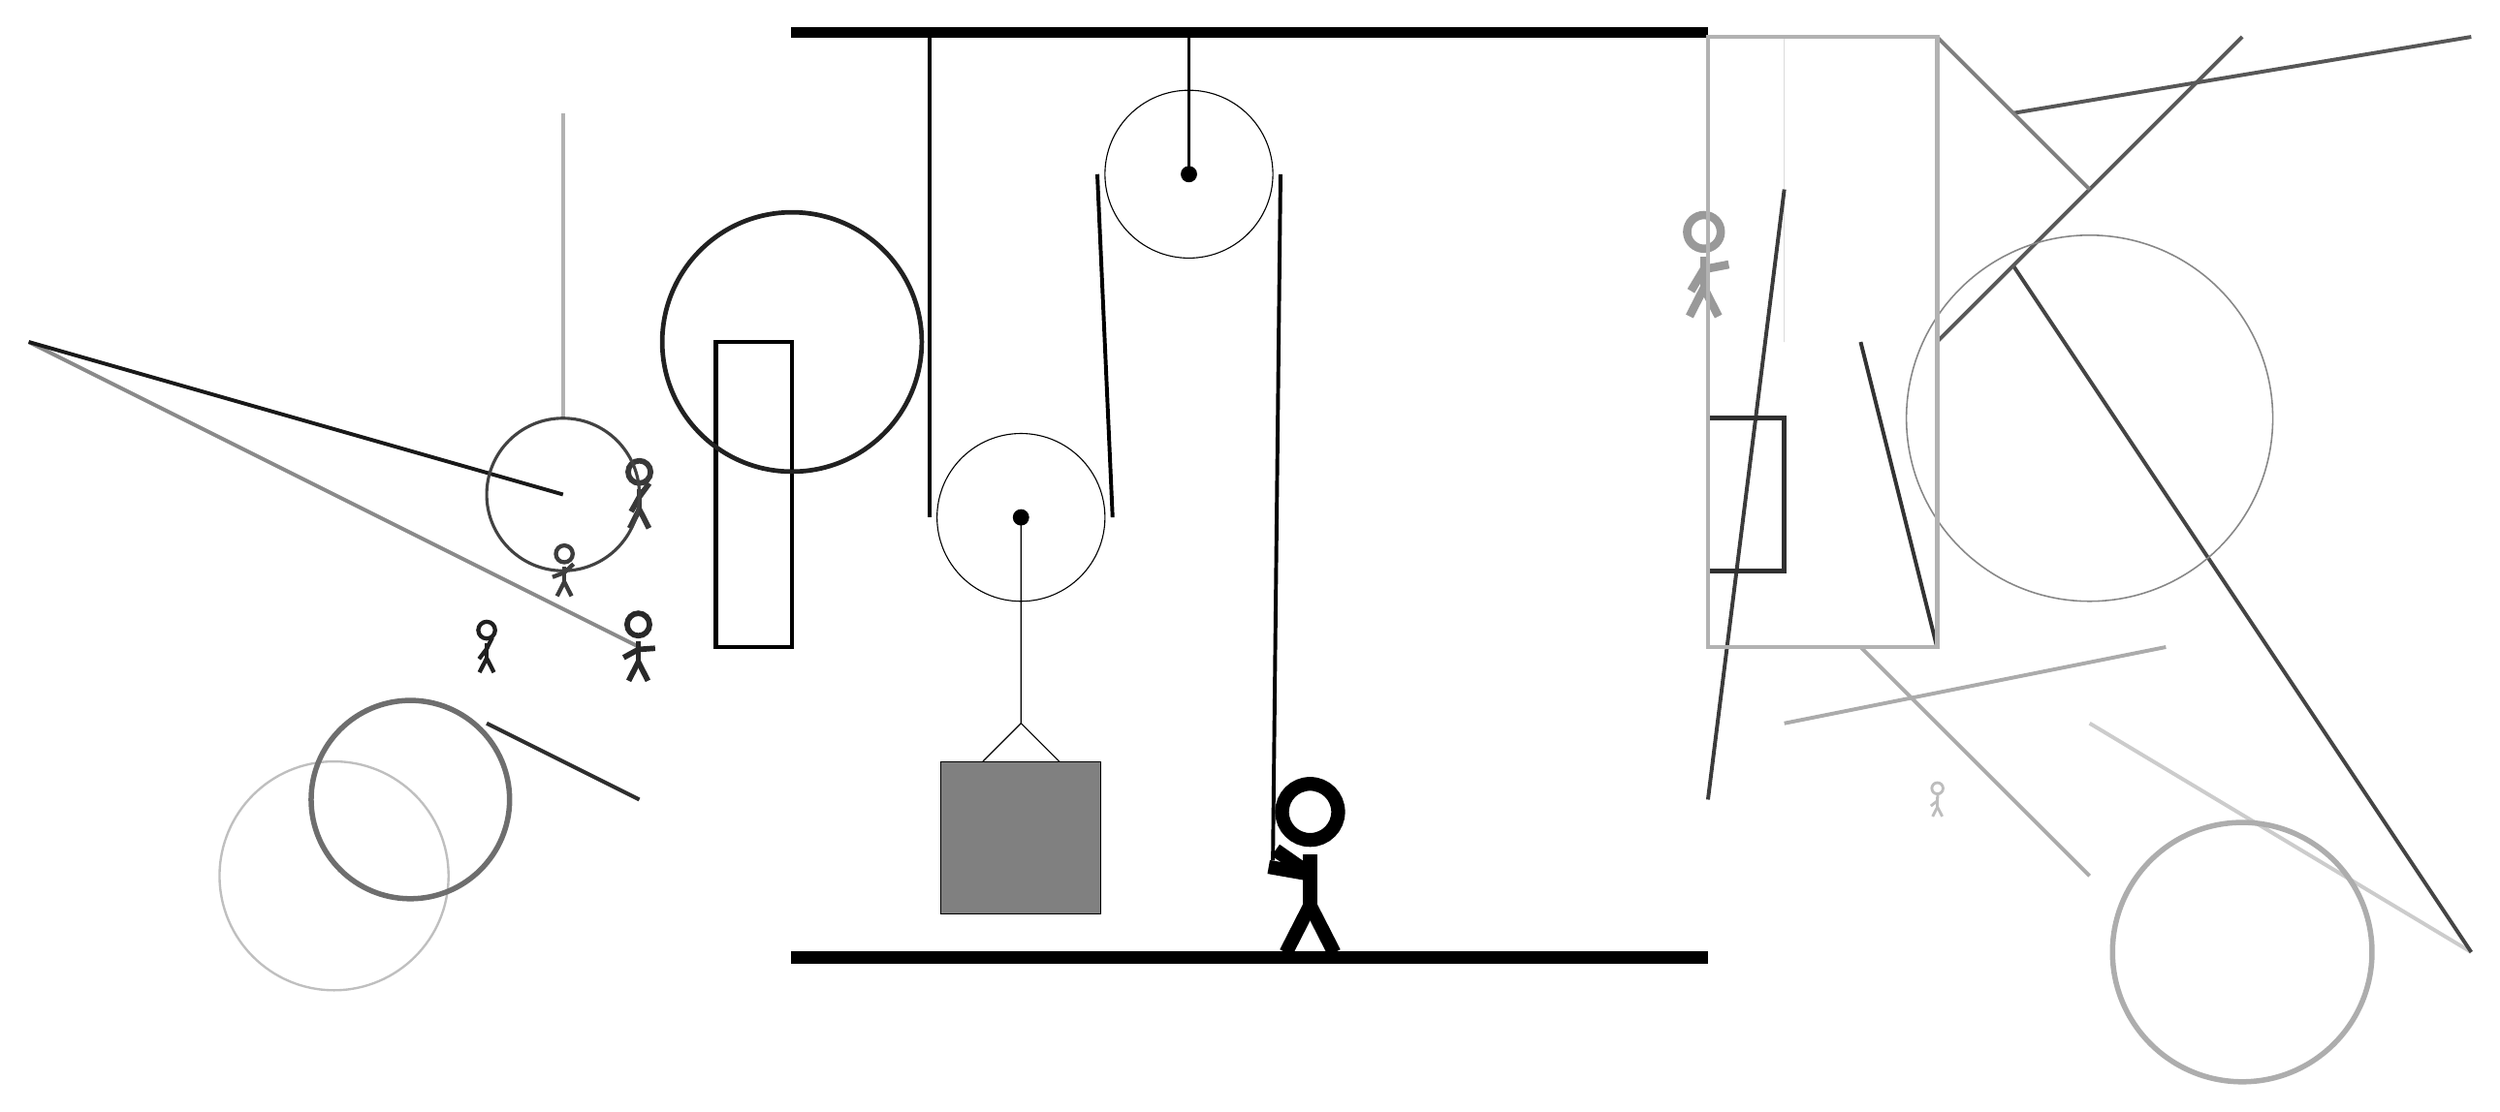
\begin{tikzpicture}
			%%%%% START %%%%%
			
			\draw[fill=black] (-2, 9) rectangle (10, 9.125);
			
			\draw[line width=0.6mm, color=black!100] (-3, 1) rectangle (-2, 5);
			
			\draw [line width=0.3mm, color=black!25](-8, -2) circle (1.5);
			\draw[line width=0.5mm, color=black!33](11, 0) -- (16, 1);
			\draw[line width=0.2mm, color=black!14] (11, 5) rectangle (11, 9);
			\draw [line width=0.7mm, color=black!57](-7, -1) circle (1.3);
			\draw[line width=0.5mm, color=black!77](11, 7) -- (10, -1);
			\node[line width=0.7mm, color=black!88] at (-6, 1) {\Strichmaxerl[3][53][64]};
			
			\draw[line width=0.5mm, color=black!33](15, -2) -- (12, 1);
			\draw[line width=0.5mm, color=black!80](12, 5) -- (13, 1);
			\node[line width=0.7mm, color=black!76] at (-5, 2) {\Strichmaxerl[3][21][43]};
			\draw[line width=0.6mm, color=black!81] (10, 2) rectangle (11, 4);
			\node[line width=0.6mm, color=black!26] at (13, -1) {\Strichmaxerl[2][38][87]};
			\node[line width=0.2mm, color=black!78] at (-4, 3) {\Strichmaxerl[4][61][54]};
			
			\draw[line width=0.5mm, color=black!46](-4, 1) -- (-12, 5);
			\draw[line width=0.5mm, color=black!90](-5, 3) -- (-12, 5);
			\node[line width=0.7mm, color=black!40] at (10, 6) {\Strichmaxerl[6][59][11]};
			
			\node[line width=0.7mm, color=black!84] at (-4, 1) {\Strichmaxerl[4][29][4]};
			\draw[line width=0.5mm, color=black!30](-5, 8) -- (-5, 4);
			\draw[line width=0.5mm, color=black!20](15, 0) -- (20, -3);
			
			\draw [line width=0.7mm, color=black!32](17, -3) circle (1.7);
			\draw[line width=0.5mm, color=black!66](14, 8) -- (20, 9);
			
			\draw [line width=0.6mm, color=black!51](14, 2) circle (0.0);
			\draw [line width=0.6mm, color=black!87](-2, 5) circle (1.7);
			\draw[line width=0.5mm, color=black!73](14, 6) -- (20, -3);
			\draw[line width=0.5mm, color=black!65](13, 5) -- (17, 9);
			
			\draw [line width=0.4mm, color=black!74](-5, 3) circle (1.0);
			\draw[line width=0.5mm, color=black!50](13, 9) -- (15, 7);
			\draw [line width=0.2mm, color=black!47](15, 4) circle (2.4);
			\draw[line width=0.6mm, color=black!30] (10, 9) rectangle (13, 1);
			
			\draw[line width=0.5mm, color=black!82](-6, 0) -- (-4, -1);
			
			\draw (3.2, 7.2) circle (1.1);
			\draw[fill=black] (3.2, 7.2) circle (0.1);
			\draw[thick] (3.2, 7.2) -- (3.2, 9);
			
			\draw (1, 2.7) circle (1.1);
			\draw[fill=black] (1, 2.7) circle (0.1);
			
			\draw (1, 2.7) -- (1, 0) -- (0.5, -0.5);
			\draw (1, 0) -- (1.5, -0.5);
			\draw[fill=black!50] (-0.05, -0.5) rectangle (2.05, -2.5);
			
			\draw[line width=0.5mm] (-0.2, 9) -- (-0.2, 2.7);
			\centerarc[line width=0.5mm](1, 2.7)(180:360:1.2000000000000002);
			\draw[line width=0.5mm](2.2, 2.7) -- (2.0, 7.2);
			\centerarc[line width=0.5mm](3.2, 7.2)(0:180:1.2000000000000002);
			\draw[line width=0.5mm](4.4, 7.2) -- (4.3, -1.8);
			
			\node at (4.7, -1.9) {\Strichmaxerl[10][-35][170]};
			
			\draw[fill=black] (-2, -3) rectangle (10, -3.15);
			
			%%%%% END %%%%%
		\end{tikzpicture}
	\end{figure}	
\end{document}